\documentclass{beamer}
\setbeamertemplate{caption}[numbered]
\usepackage{animate, lipsum, subfig}
\usepackage{subfig}


\newcommand{\comment}[1]{}

\newcommand\blfootnote[1]{%
  \begingroup
  \renewcommand\thefootnote{}\footnote{#1}%
  \addtocounter{footnote}{-1}%
  \endgroup
}

% Load Packages
\usepackage[utf8]{inputenc}
\usepackage{xcolor}
\usepackage{tikz}
\usetikzlibrary{positioning,calc}
\usepackage{graphicx}
\usepackage{hyperref}
\usepackage{amsmath}
\usepackage{listings}
%\usepackage{fontawesome}

% Define Commands
\newcommand*{\ClipSep}{0.06cm} %To adjust footer logo
\newcommand{\E}{\mathrm{e}\,} %\def\I{e} % used to defined e for exp(x), see later what it should be
\newcommand{\ud}{\mathrm{d}}
\lstset{numbers=left, numberstyle=\tiny, stepnumber=1,firstnumber=1,breaklines=true,
    numbersep=5pt,language=Python,
    stringstyle=\ttfamily,
    basicstyle=\footnotesize, 
    showstringspaces=false
}

\usetheme{oxonian}

\title{LXe scintillation model}
\begin{document}

{\setbeamertemplate{footline}{} 
\frame{\titlepage}}

\begin{frame}{Objective}
The goal is build a scintillation model for LXe: $Y_{a}(t,\hat{\theta})$.\\
$Y_{a}(t,\hat{\theta})$ is the probability to emit a photon at time $t$ to the direction $\hat{\theta}$. The subscript $a$ indicates the different type of interactions ($\gamma$, $N$, $\alpha$ and maybe different energies in the same interaction type).\\

For that 4 measurements were made 2 with $^{57}$Co (122 KeV $\gamma$s) and 2 with $^{137}$Cs (662 KeV $\gamma$s). The 2 measurements with the same source were done with 90$^\circ$ rotation, one relative to the other.
\end{frame}


\begin{frame}{Signal Reconstruction}
%	\begin{center}
%	\animategraphics[loop,controls,width=0.6\linewidth]{10}{recon-}{0}{41}	
%	\end{center}
To study the temporal structure of the photon emission a processing algorithm uses a template of the average SPE signal to reconstruct the temporal PE pattern in each event for each PMT separately. The output of this process is the number of PEs created in the PMT in each digitization point. These temporal patters are aligned by the first PE in each event.

\begin{figure}[h]
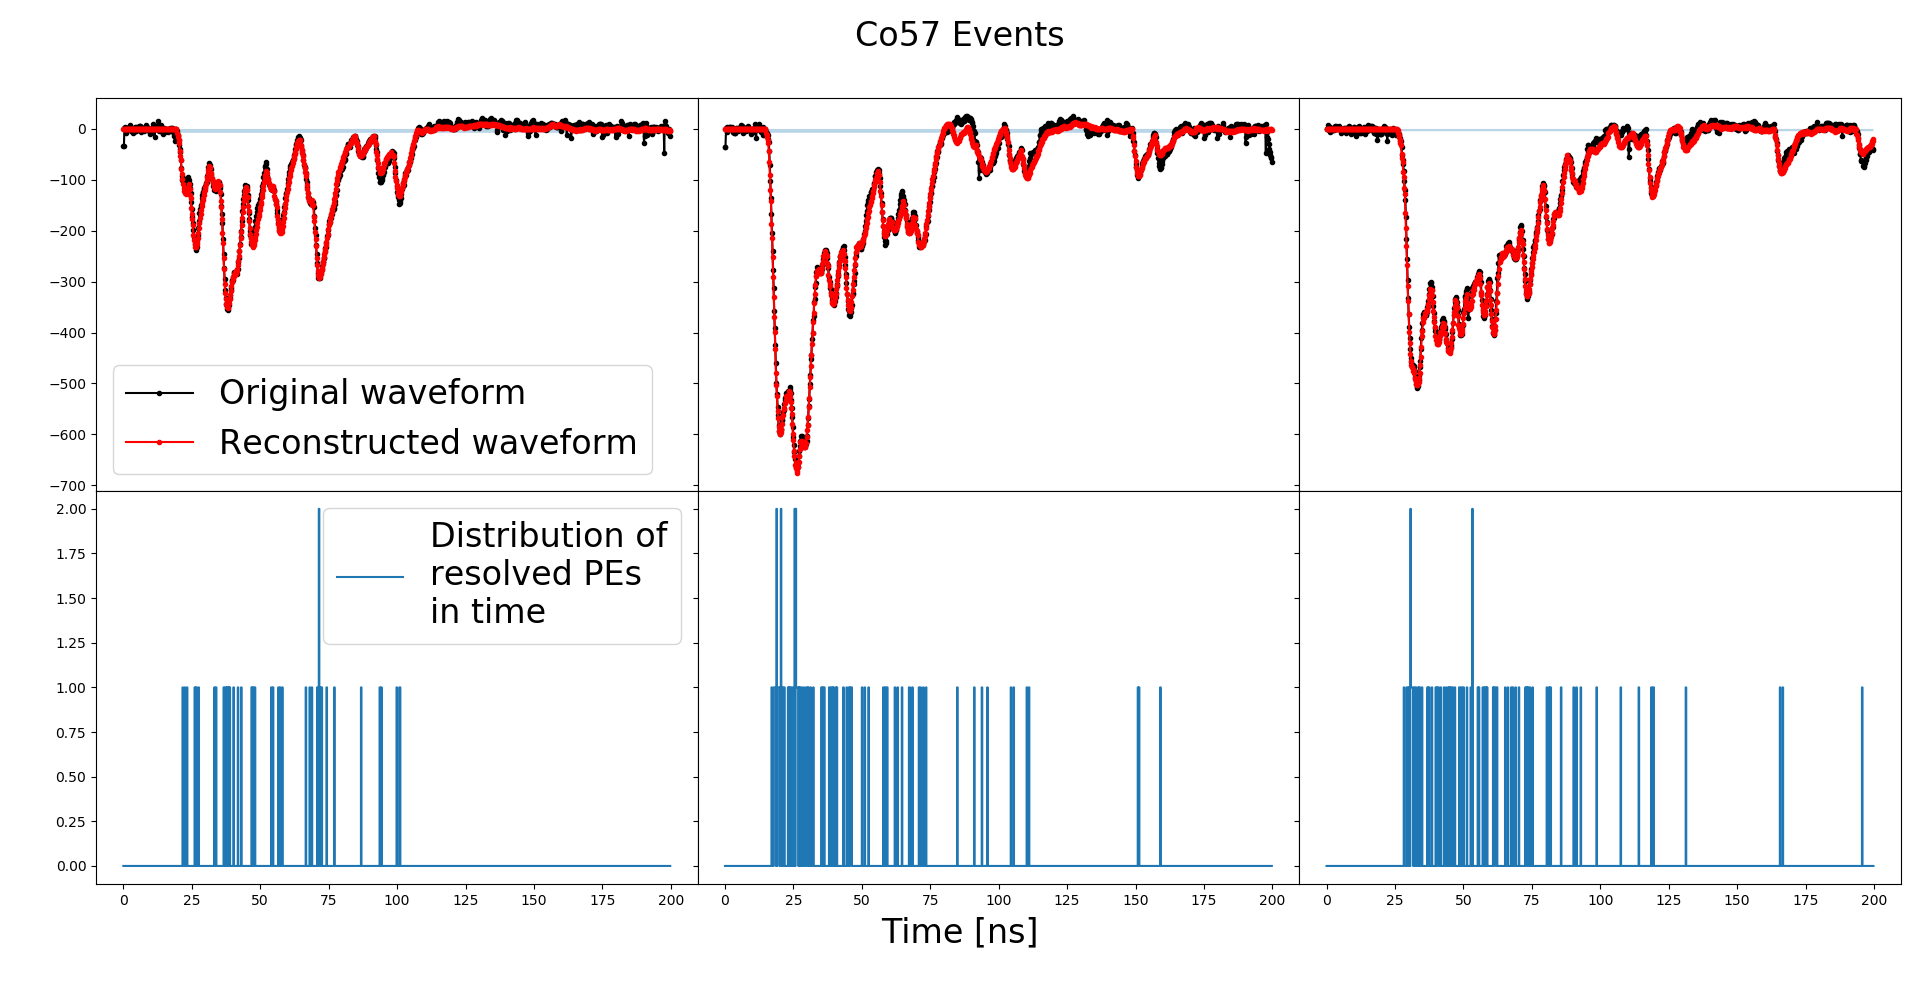
\includegraphics[width=1\textwidth]{recons.png}
\end{figure}
\end{frame}

\begin{frame}{SPE Calibration}

\end{frame}

\begin{frame}{Event Reconstruction Algorithm}

\end{frame}

\begin{frame}{Data Selection - PMT flashing}
After reconstruction some quality cuts are made ($\chi^2$, blw and first PE). Then also PMT fleshing events are cut out. This events are characterized by the amount of the PEs in the first 10 ns of the event relative to full amount of the PEs ($\omega$). Events with $\omega>0.5$ are cut out. This events assumed to be generated by the PMTs because such events were found also when there were no sphere in the setup (both Co and Cs datasets gives $0.15$~Hz of PMT fleshing). 
\begin{figure}[h]
    \centering
    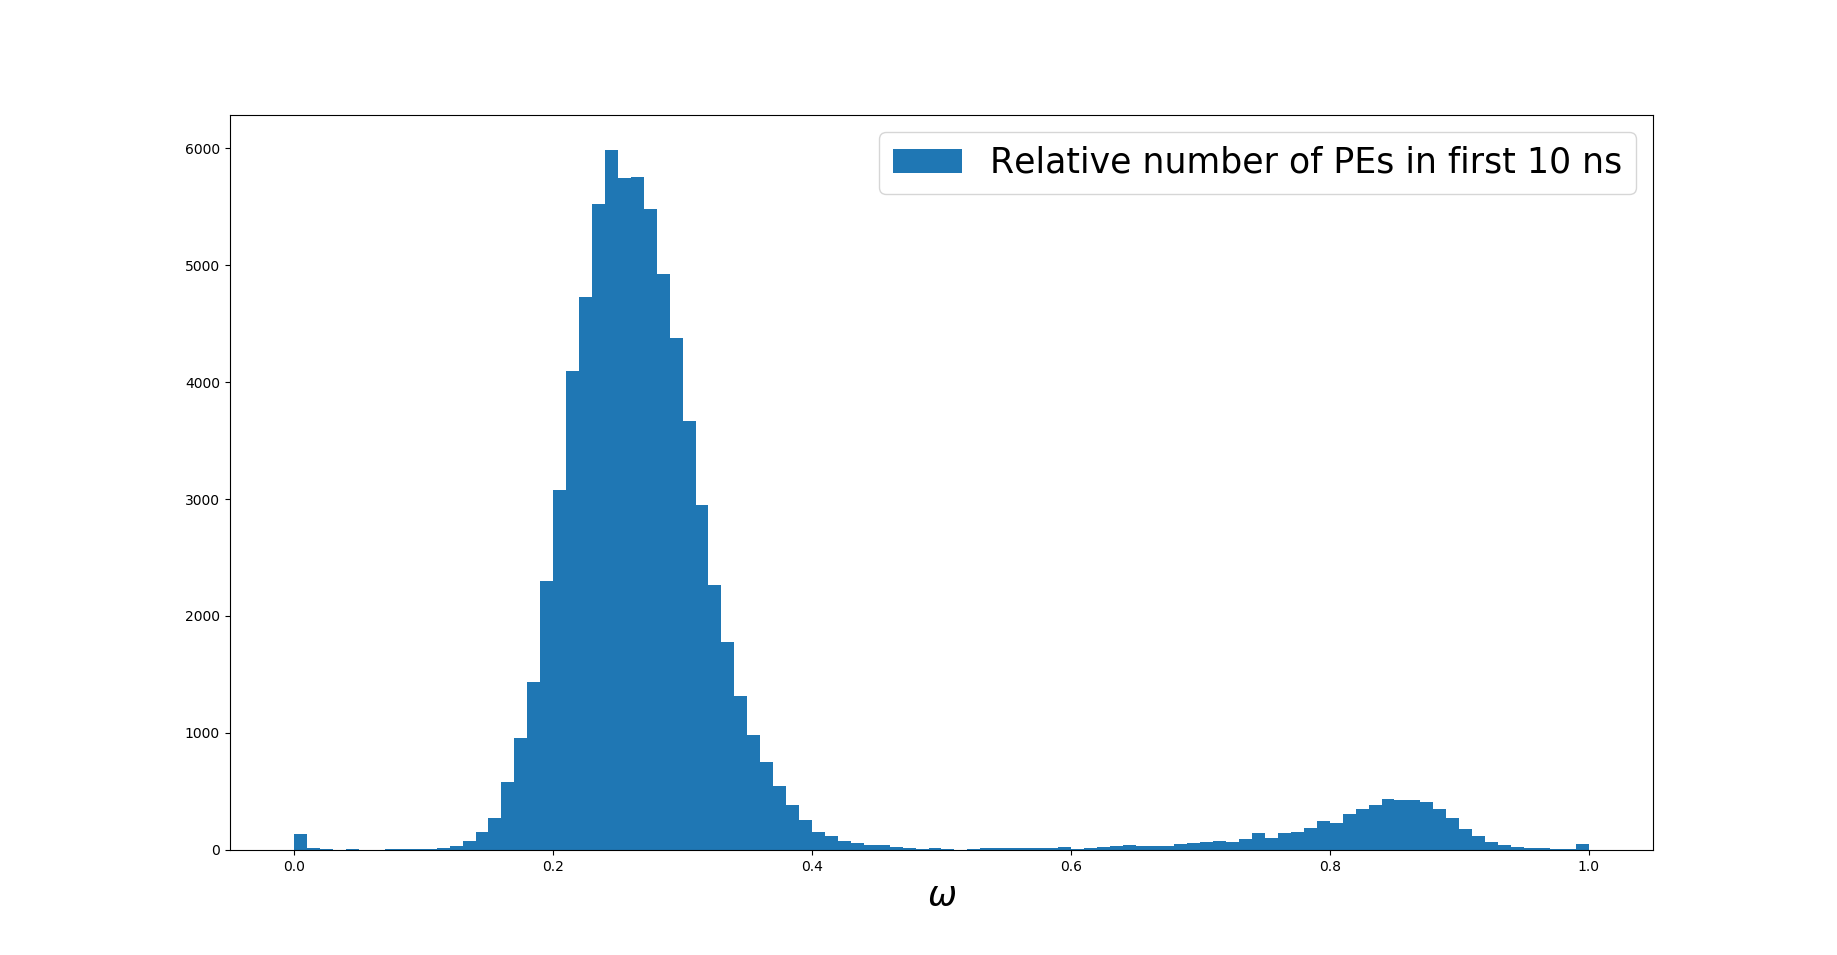
\includegraphics[width=0.75\textwidth]{w.png}
\end{figure}
\end{frame}

\begin{frame}{Data Selection - Spectrum}
\begin{figure}
Finally, only events around the full absorption peak were chosen
\subfloat[$^{57}$Co]{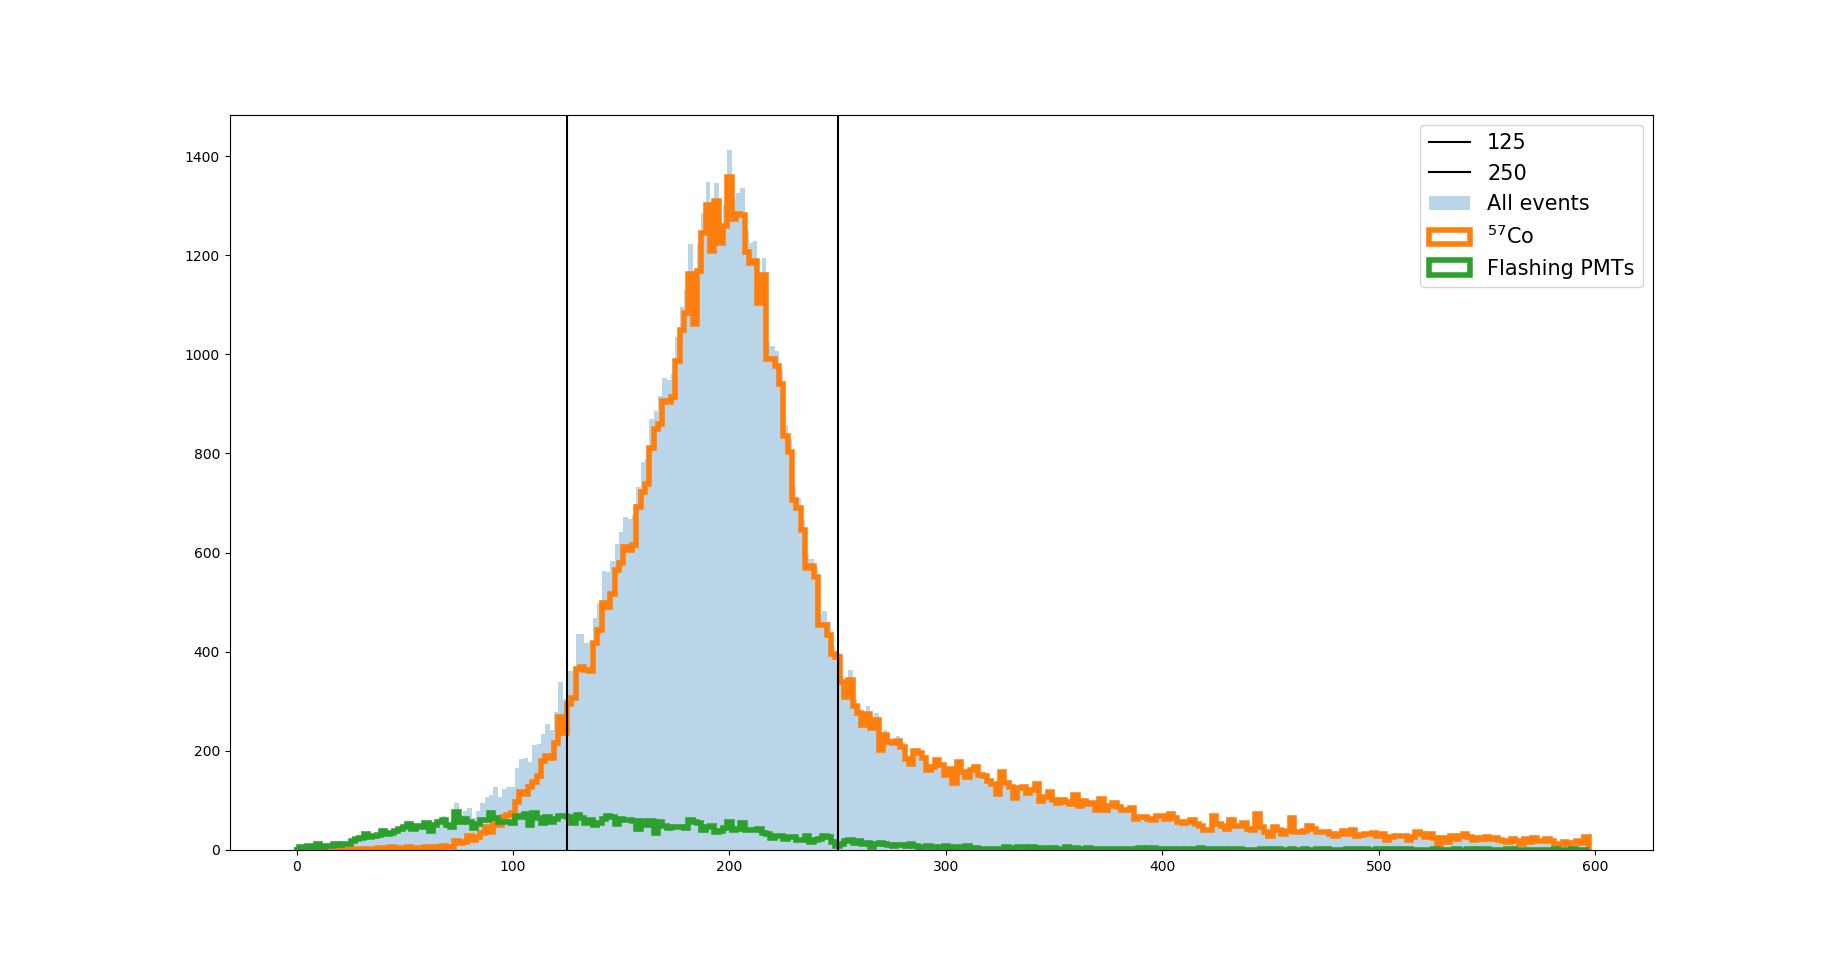
\includegraphics[width=0.5\textwidth]{Co57.png}}\qquad
  \subfloat[$^{137}$Cs]{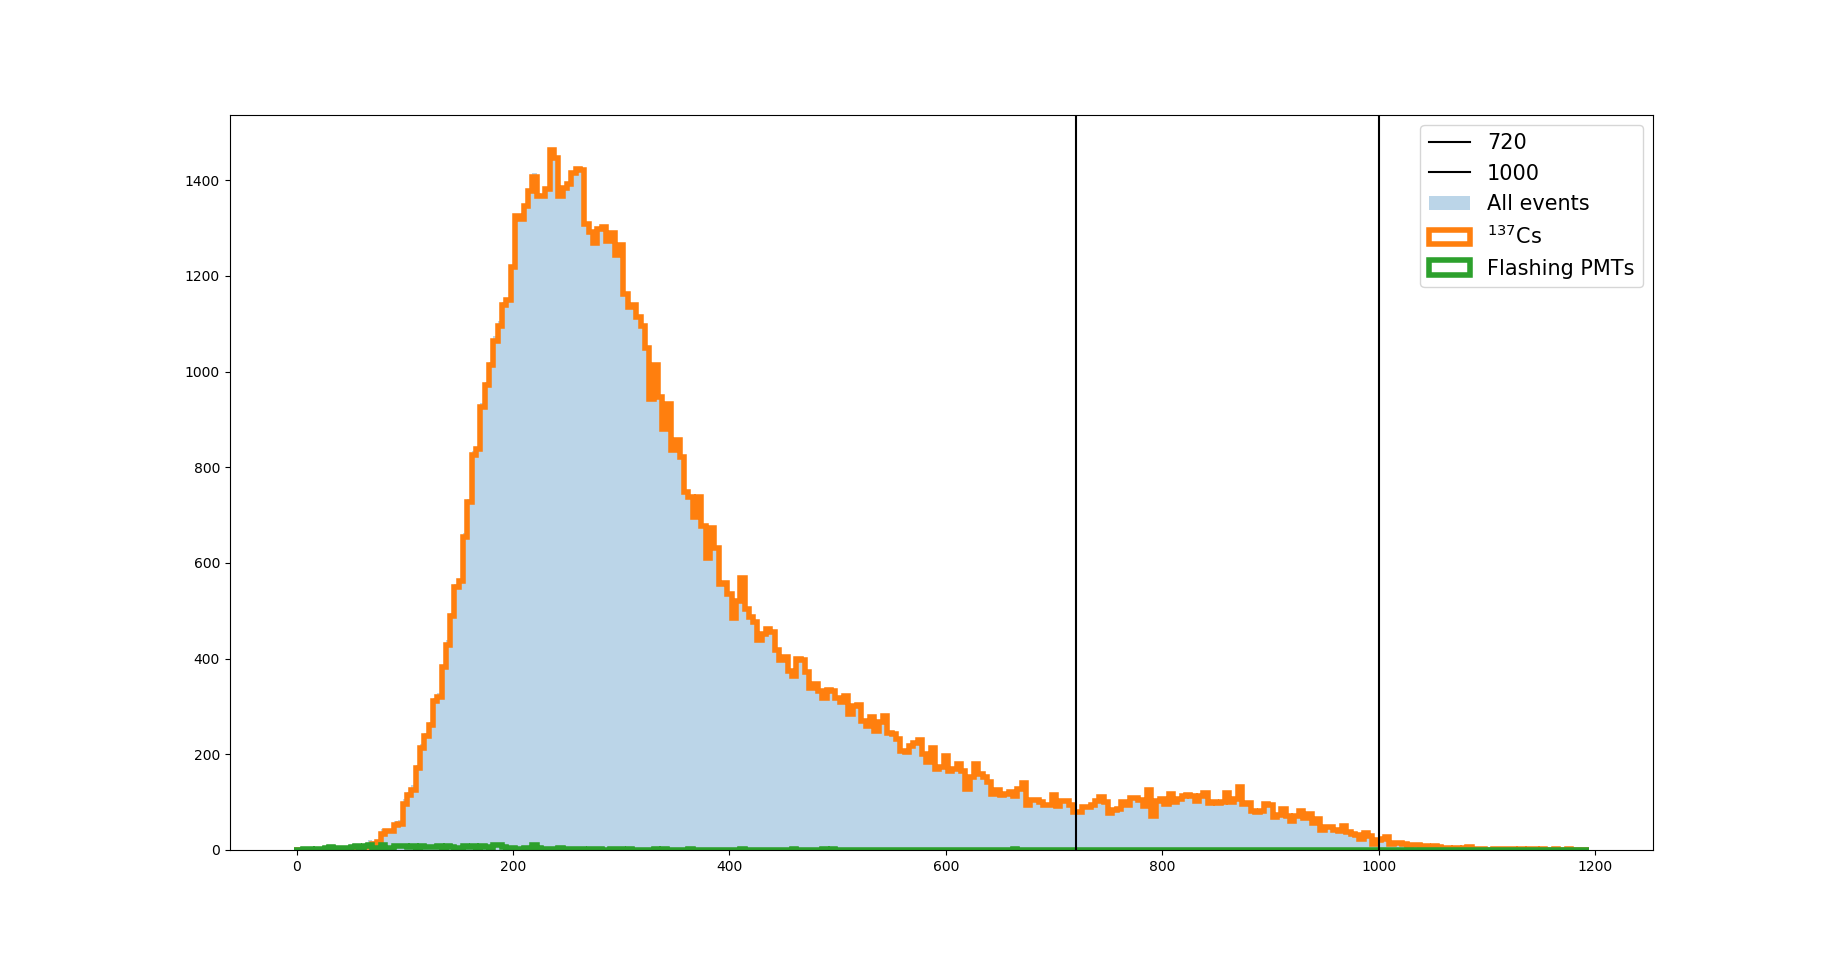
\includegraphics[width=0.5\textwidth]{Cs137.png}}
\end{figure}
\end{frame}

\begin{frame}{Average Temporal Structure}
\begin{figure}[h]
    \centering
    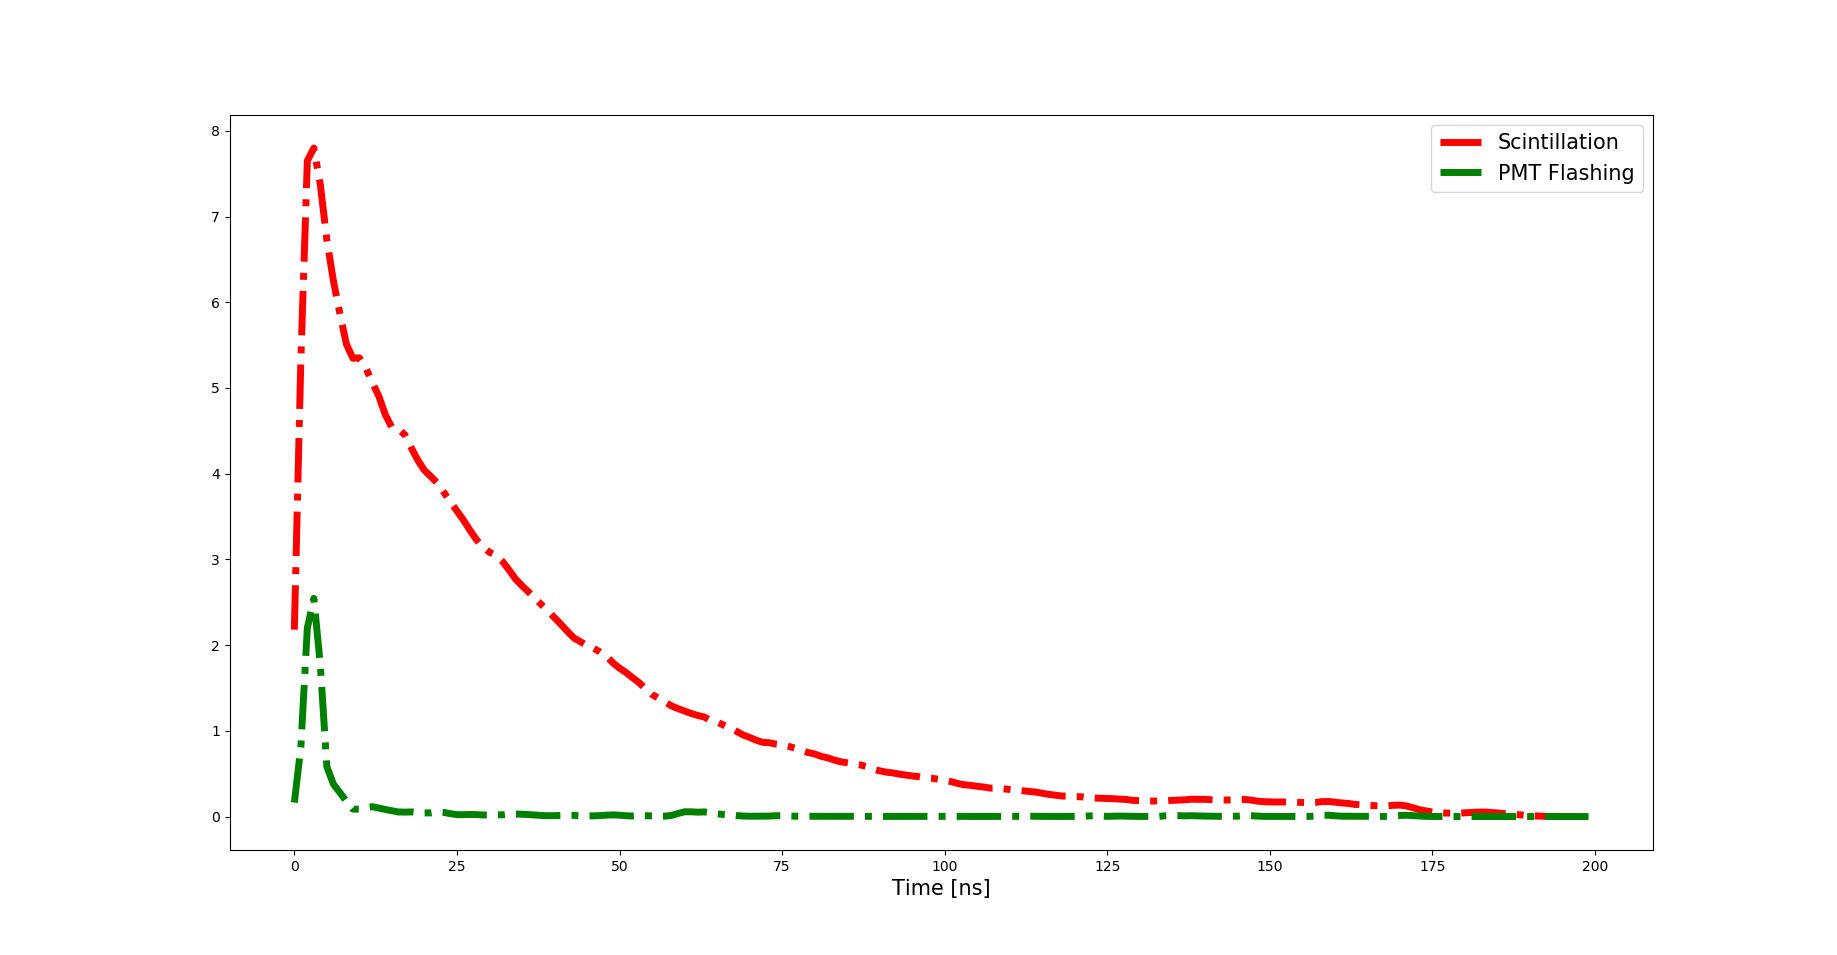
\includegraphics[width=1\textwidth]{temp.png}
\end{figure}
\end{frame}

\begin{frame}{The Dataset $D_{\nu ia}$}
For each measurement a 3D table ($D_{\nu ia}$) is build. It holds the number of events in which $n$ PEs were resolved at time $i$ (after the first PE in the events) in PMT $a$.\\

A 3D array is build ($H_{\nu ia}$) using a scintillation model and PMT parameters and is fitted to $D_{\nu ia}$.
\end{frame}


\begin{frame}{Scintillation Model}
The probability that $\nu$ PEs were resolved at time window $[t_i-dt/2, t_i+dt/2]$ by PMT $a$, given that $n$ photons were created at the event is
\begin{equation}
B_{\nu ian}=\text{Binom}(\nu|n,d\Omega_aQ_adtY_{i})
\end{equation}
where $d\Omega_a$ and $Q_a$ are the solid angle and the light detection efficiency of PMT $a$ and $Y_i$ is the probability to emit a photon at time window $i$.

\blfootnote{Light detection efficiency is all the mechanisms which generates $m$ PEs from $n>m$ photons that hit the face of the PMT. This includes quantum efficiency, collection efficiency, double PE probability and more}
\end{frame}

\begin{frame}{Scintillation Model - Time Smearing}
Each PMT has its temporal resolution ($\sigma_a$) and a delay ($T_a$).
This means that a PE that was created at time $i$ has a probability to be resolved at time $j$. This probability is
\begin{equation}
P_{ij}=\frac{dt}{\sqrt{(2\pi)\sigma_a}}e^{-(t_j-t_i-T_a)^2/2\sigma_a^2}
\end{equation}
Thus
\begin{equation}
Y_i\rightarrow Y_{ja}=\int_0^{\infty}Y_{t_i}\frac{dt}{\sqrt{(2\pi)\sigma_a}}e^{-(t_j-t_i-T_a)^2/2\sigma_a^2}
\end{equation}

\end{frame}

\begin{frame}{Scintillation Model - Alignment by the First PE}
The probability that PMT $a$ will resolve $\nu>0$ PEs at the same time window as the first PE in the event (this goes to $H_{\nu0a}$), given that $n$ photons were created at the event is
\begin{equation}
P_{\nu0a}=\sum_j\prod_{k<j}\prod_bB_{0kbn}B_{\nu jan}.
\end{equation}
To get the model for the 3D array the number of the photons per event needs to be averaged
\begin{equation}
H_{\nu0a}=\sum_{j,n}\prod_{k<j}\prod_bB_{0kbn}B_{\nu jan}\text{Poisson}(n|N)
\end{equation}
were $N$ is the average number of photons created in the interaction.
\end{frame}

\begin{frame}{Scintillation Model - Alignment by the First PE}
The probability that PMT $a$ will resolve $0$ PEs at the same time window as the first PE in the event (this goes to $H_{00a}$), given that $n$ photons were created at the event is
\begin{equation}
P_{00a}=\sum_j\prod_{k<j}\prod_bB_{0kbn}(1-\prod_cB_{0jcn})B_{0jan}.
\end{equation}
So
\begin{equation}
H_{00a}=\sum_{j,n}\prod_{k<j}\prod_bB_{0kbn}(1-\prod_cB_{0jcn})B_{0jan}\text{Poisson}(n|N)
\end{equation}
\end{frame}


\begin{frame}{Scintillation Model - Alignment by the First PE}
The probability that PMT $a$ will resolve $\nu$ PEs at time window $i$ after the first PE in the event (this goes to $H_{\nu ia}$), given that $n$ photons were created at the event is
\begin{equation}
P_{\nu ia}=\sum_j\prod_{k<j}\prod_bB_{0kbn}(1-\prod_bB_{0jbn})B_{\nu j+ian}.
\end{equation}
So
\begin{equation}
H_{\nu0a}=\sum_j\prod_{k<j}\prod_bB_{0kbn}(1-\prod_bB_{0jbn})B_{\nu j+ian}\text{Poisson}(n|N)
\end{equation}
\end{frame}

\begin{frame}{Scintillation Model}
Take $Y_i$ as a sum exponential decaying components
\begin{equation}
Y_a(t_j)=\sum_c\frac{F_c}{\tau_c}e^{-t_j/\tau_c} \quad (\sum_cF_c=1)
\end{equation}
we will get 
\begin{equation}
\begin{split}
&\int Y_a(t_j)\text{Norm}(t_i|T_0+t_j, \sigma_t)dt=\\
&\sum_c\frac{F_cK_c}{\tau_c}e^{-t_i\tau_c}\left[1-\text{erf}\left(\frac{\sigma_t}{\sqrt{2}\tau_c}-\frac{t_i-T_0}{\sqrt{2}\sigma_t}\right)\right]
\end{split}
\end{equation}
where $K_c$ is a normalization factor
\begin{equation}
K=\left[1-\text{erf}\left(\frac{\sigma_t}{\sqrt{2}\tau}+\frac{T_0}{\sqrt{2}\sigma_t}\right)+e^{-\sigma_t^2/2\tau^2-T_0/\tau}\left(1+\text{erf}\left(\frac{T}{\sqrt{2}\sigma_t}\right)\right)\right]^{-1}
\end{equation}
\end{frame}

\begin{frame}{Scintillation Model with $\delta(t)$}
If we want to add a super fast component in the beginning of the model it is represented by
\begin{equation}
Y_a(t)=(1-R_\delta)\sum_c\frac{F_c}{\tau_c}e^{-t/\tau_c}+R_\delta\delta(t),
\end{equation}
So we need to add to equation 8 from the previous slide:
\begin{equation}
\frac{R_\delta}{\sqrt{2\pi}\sigma_t}e^{-(t-T_0)^2/(2\sigma_t^2)}
\end{equation}
\end{frame}

\begin{frame}{Scintillation Model - Alignment}
Recall that we build a model for $H_{ni}$ which holds the number of events in which $n$ PEs were resolved at time $t_i$ after the first resolved PE.
Without the alignment problem, naively, 
\begin{equation}
\tilde{H}_{ni}=N_{\text{events}}\text{Poisson}\left(n\bigg|\lambda=QN_adt\int Y_a(t_j)\text{Norm}(t_i|T_0+t_j, \sigma_t)dt\right)
\end{equation}
\blfootnote{$\tilde{H}_{ni}$ is $H_{ni}$ before the alignment. The naively comment states that we also need to account the uncertainty in the number of PEs resolved, i.e the probability to resolve $n$ PEs where $m$ where actually extracted. This is related to the width of the SPE area distribution  and will be treated later.}
\end{frame}

\begin{frame}{Alignment for $i>0$}
The model $\tilde{H}_{ni}$ tells us what is the probability that $n$ PEs will be resolved at time $t_i$. So 
\begin{equation}
\begin{split}
H_{ni}=\sum_j&[\text{Non of the PMTs resolved a PE untill time }t_j]\times\\
&[\text{Some PMT resolved a PE (or more) at time }t_j]\times\\
&\tilde{H}_{ni+j}
\end{split}
\end{equation}
\end{frame}

\begin{frame}{Alignment for $i>0$}
\begin{equation}
\begin{split}
&[\text{Non of the PMTs resolved a PE untill time }t_j]=\\
&\prod_{\text{all PMTs}}\prod_{k<j}\tilde{H}_{0k}^{\text{pmt}}
\end{split}
\end{equation}
\begin{equation}
\begin{split}
&[\text{Some PMT resolved a PE (or more) at time }t_j]=\\
&1-\prod_{\text{pmt}}\tilde{H}_{0j}^{\text{pmt}}
\end{split}
\end{equation}

\blfootnote{The superscript pmt indicates the product on all PMTs (each pmt has a different model).}
\end{frame}

\begin{frame}{Alignment for $i>0$}
\begin{equation}
H_{ni}=\sum_j\prod_{\text{all PMTs}}\prod_{k<j}\tilde{H}_{0k}^{\text{pmt}}\left(1-\prod_{\text{pmt}}\tilde{H}_{0j}^{\text{pmt}}\right)\tilde{H}_{ni+j}
\end{equation}
\end{frame}

\begin{frame}{Alignment for $i=0, n>0$}
In this case we dont need the middle term in the previous slide (which represents the probability that the first PE was resolved at time $t_j$), So for $n>0$
\begin{equation}
H_{n0}=\sum_j\prod_{\text{all PMTs}}\prod_{k<j}\tilde{H}_{0k}^{\text{pmt}}\tilde{H}_{nj}
\end{equation}
\end{frame}

\begin{frame}{Alignment for $i=0, n=0$}
Here we do need the middle term but we dont want to sum on the pmt of interest. So
\begin{equation}
H_{00}^{\text{pmt}_0}=\sum_j\prod_{\text{all PMTs}}\prod_{k<j}\tilde{H}_{0k}^{\text{pmt}}\left(1-\prod_{\text{pmt}\neq\text{pmt}_0}\tilde{H}_{0j}^{\text{pmt}}\right)\tilde{H}_{0j}^{\text{pmt}_0}
\end{equation}
\end{frame}

\begin{frame}{Event Simulation}
the simulation creates the temporal structure of 10K events on two PMTs. Align the events by the first PE and finally creates a simulated 2D table for each PMT ($S_{ni}$) which holds the number of simulated events in which $n$ PEs were created at time $t_i$ after the first PE in the event. 
For each simulated event:
\begin{itemize}
\item A trigger time ($t_{trig}$) is randomly chosen from a normal distribution with mean 0 and variance $\sigma_{trig}^2$. This trigger is common for all PMTs.
\item For each PMT a total number of PEs in event ($n$) is randomly chosen out of a Poisson distribution with mean $NQ$.
\item For each PMT the $n$ PEs are grouped in two groups $n_f, n_s$ (three groups with $n_\delta$ if we want to simulate a $\delta(t)$ pulse). The occupancy of each group chosen randomly from distribution with probabilities $F, 1-F$ (and $R_\delta^a$ for the $\delta$ model). 
\end{itemize}
\end{frame}

\begin{frame}{Event Simulation}
\begin{itemize}
\item For each PMT, $nf$ times ($t_f$) are randomly chosen from an exponential distribution with decay constant $\tau_f$, and $ns$ times ($t_s$) are randomly chosen from an exponential distribution with decay constant $\tau_s$.
\item For each PMT we smear the two exponential component by shifting each sampled time $t_{f/s}^i\rightarrow \text{Normal}(\text{mean}=t_{trig}+T_0^a+t_{f/s}^i, \text{Var}=(\sigma_t)^2)$, where $\sigma_t$ is the temporal uncertainty of the PMT.
\item Find the minimal time over all PMTs (global for event) and roll all times back relative to this time.
\end{itemize}
\end{frame}

\begin{frame}{First Look at Data}
I ran the reconstruction algorithm on the $^{57}$Co dataset with PMTs 7 and 8. In each event the two signals were aligned by the delay that was measured by the pulser data. After reconstruction the temporal pattern of the resolved PEs was aligned ones more relative to the first PE resolved (in PMT 7 or 8). The events in which the $\chi^2$ of the reconstructed signal relative to the signal was too big were cut out. Also events with large baseline width were cut out. A range in the energy spectrum (number of resolved PEs) of each PMT was chosen and from these events a 2D table was made for each PMT ($D_{ni}$) which holds the number of events in which $n$ PEs was resolved at time $t_i$ after the first resolved PE.
\end{frame}


\end{document}

